\documentclass[a4paper,10pt]{ltjsarticle}
\usepackage[top=17mm,bottom=18mm,left=19mm,right=19mm]{geometry}
\usepackage{graphicx,booktabs,tabularx,array,float,amsmath,amssymb,xcolor}
\usepackage{tikz}
\usetikzlibrary{arrows.meta,positioning}
\usepackage[unicode,hidelinks]{hyperref}
\usepackage{fancyvrb}
\hypersetup{pdftitle={CylinderTag検出改善と処理パイプライン},pdfauthor={Codex}}
\definecolor{accent}{HTML}{167B55}
\definecolor{muted}{HTML}{555555}
\setlength{\parindent}{1em}
\setlength{\parskip}{3pt}
\setlength{\abovecaptionskip}{4pt}
\renewcommand{\arraystretch}{1.2}
\newcommand{\fig}[2]{\includegraphics[width=#1]{generated/#2}}
\newcommand{\smallnote}[1]{{\small\color{muted}#1}}
\input{generated/metrics.tex}
\begin{document}
\begin{center}
{\LARGE\bfseries CylinderTag 検出アルゴリズムの改善}\\[3mm]
{\large 印刷試験片の動画解析と処理パイプラインの可視化}\\[2mm]
2026年10月18日\quad 原動画：ユーザー提供\quad 解析・実装：Codex
\end{center}

\section*{1. 結果と評価対象}
白黒 PLA の薄い試験片を円筒に貼った動画 \texttt{IMG\_2422.mov} を対象に、
候補抽出から辞書照合までを改善した。結果は\textbf{ID 0 の出力が
\BeforeCount/\FrameCount\ から \AfterCount/\FrameCount\ フレームに増加}し、
別 ID の出力は \BeforeWrong\ から \AfterWrong\ フレームに減少した。
追跡による補間や、直前の ID を表示し続ける処理は使っていない。

\begin{table}[H]\centering
\begin{tabular}{lrr}\toprule
指標 & 従来版 & 改善版\\\midrule
入力フレーム数 & \FrameCount & \FrameCount\\
ID 0 が出たフレーム & \BeforeCount\ (\BeforeRate\%) & \AfterCount\ (\AfterRate\%)\\
別 ID が出たフレーム & \BeforeWrong & \AfterWrong\\
ID 0 が出なかったフレーム & 265 & 96\\\bottomrule
\end{tabular}
\caption{同一動画の全フレーム比較。率の分母は266フレーム。}
\end{table}

\begin{figure}[H]\centering
\begin{minipage}{.43\linewidth}\centering
\fig{.86\linewidth}{before.png}\\\small 従来版：ID が出ない
\end{minipage}\hspace{6mm}
\begin{minipage}{.43\linewidth}\centering
\fig{.86\linewidth}{after.png}\\\small 改善版：ID 0、鏡像として照合
\end{minipage}
\caption{同じ frame 87（約3.01秒）。表示領域だけを同一範囲で切り出した。}
\end{figure}

\textbf{主な原因は三つあった。}
(1) 入力の強制1/2縮小による細い模様の情報損失、
(2) 初版 STL の鏡像、(3) 列の幾何判定と辞書照合の不具合である。
しきい値だけを緩めると別 ID も採用しやすくなるため、
候補を拾う処理と、曖昧な ID を棄却する処理を分けた。

\smallnote{入力は480\,$\times$\,854、266フレーム、約9.205秒。
期待 ID は生成元の辞書から0とした。本動画を開発にも使用しているため、
この率は未知の撮影条件に対する汎化性能ではない。物理位置・姿勢の精度も測っていない。}

\clearpage
\section*{2. 処理パイプラインと実際の中間画像}
ArUco の輪郭候補抽出・局所二値化・射影正規化、および AprilTag の
辺に沿った勾配の集約という考え方を、CylinderTag の列構造へ適用した\cite{aruco,apriltag2,apriltagcode}。
円筒全体を一枚の平面に変換するのではなく、各列の外側四点を個別に正規化する。

\begin{figure}[H]\centering
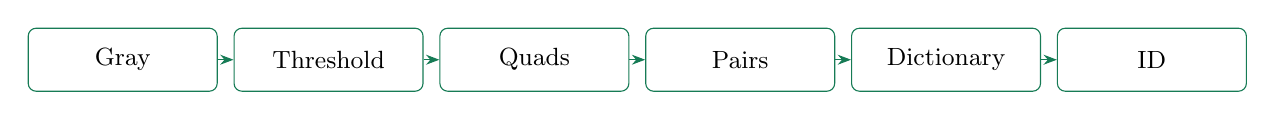
\begin{tikzpicture}[node distance=2mm,box/.style={draw=accent,rounded corners=1mm,minimum width=24mm,minimum height=8mm,font=\small},>=Stealth]
\node[box] (a) {Gray};
\node[box,right=of a] (b) {Threshold};
\node[box,right=of b] (c) {Quads};
\node[box,right=of c] (d) {Pairs};
\node[box,right=of d] (e) {Dictionary};
\node[box,right=of e] (f) {ID};
\foreach \x/\y in {a/b,b/c,c/d,d/e,e/f}{\draw[->,accent] (\x)--(\y);}
\end{tikzpicture}
\end{figure}

\begin{figure}[H]\centering
\begin{minipage}{.31\linewidth}\centering\fig{\linewidth}{pipeline_01_gray.png}\\\small ① 原寸のグレースケール\end{minipage}\hfill
\begin{minipage}{.31\linewidth}\centering\fig{\linewidth}{pipeline_02_binary.png}\\\small ② 局所二値化（黒領域が白）\end{minipage}\hfill
\begin{minipage}{.31\linewidth}\centering\fig{\linewidth}{pipeline_03_quads.png}\\\small ③ 四角形候補と辺の補正\end{minipage}
\vspace{4mm}

\begin{minipage}{.31\linewidth}\centering\fig{\linewidth}{pipeline_04_pairs.png}\\\small ④ 上下の黒領域を列へ組み立て\end{minipage}\hfill
\begin{minipage}{.31\linewidth}\centering\fig{\linewidth}{pipeline_05_groups.png}\\\small ⑤ 列群と各列の仮の符号\end{minipage}\hfill
\begin{minipage}{.31\linewidth}\centering\fig{\linewidth}{pipeline_06_decoded.png}\\\small ⑥ 全辞書との照合・採用\end{minipage}
\caption{frame 87 の実バッファ。原画像の $x=175\ldots409$, $y=225\ldots494$ を共通に切り出した。
候補段階に残る余分な形状を、最終段階では棄却している。}
\end{figure}

\small
二値化のタイル幅は5・11・21ピクセルの3通りで処理し、重複する検出は空間的に統合する。
図は最も強い候補を持つ一つのタイル幅の中間状態と、全タイル幅を統合した最終結果である。
フレーム0・62・87・131・200・250の PNG を保存した。初期段階で候補がなくなるフレームでは、
後続段階の画像は存在しないことがある。PNG と併せて、全フレームの候補数・列符号・交比も出力した。
\normalsize

\clearpage
\section*{3. しきい値以外にもあった原因}
\subsection*{3.1 初版 STL は辞書に対して鏡像だった}
MATLAB の画像座標は下向きが正、CAD を上面から見ると上向きが正になる。
初版の生成器はこの差を補正していなかったため、印刷物が元の符号模様の上下反転になっていた。
これは今回作成した STL 側の不具合であり、撮影や材料の問題ではない。
各側の符号 $s\in\{0,\dots,7\}$ は上下反転で $7-s$ へ変わり、
一列の符号 $c=8a+b$ は $63-c$ へ変わる。

\begin{figure}[H]\centering
\begin{minipage}{.47\linewidth}\centering
\fig{\linewidth}{pattern_legacy_mirrored.png}\\
\small 初版を上面から見た模様（鏡像）
\end{minipage}\hfill
\begin{minipage}{.47\linewidth}\centering
\fig{\linewidth}{pattern_corrected.png}\\
\small 修正版（元の画像辞書と同じ向き）
\end{minipage}
\caption{生成式から描いた比較図。CAD の見え方に対応させた模式的な平面表示。}
\end{figure}

現在の生成器はY軸を反転して修正した。検出器側では鏡像と通常の向きを両方評価し、
\texttt{mirrored} フラグを結果に残すため、印刷済みの試験片も評価できる。
鏡像に対応すると候補数が増えるので、後述の一致列数と候補間マージンを必要条件とした。

\subsection*{3.2 元の処理で確認した不具合}
\noindent\begin{tabularx}{\linewidth}{@{}p{39mm}X@{}}\toprule
箇所 & 問題と修正\\\midrule
画像端の二値化 & タイルの端のしきい値が未初期化だった。近傍の最小値・最大値を形態演算で全域へ設定した。\\
列ごとの符号判定 & 交比がどの区間にも入らない場合、直前の列の符号が残っていた。各列を独立に測定する方式へ置換した。\\
右側の幾何判定 & 右側の判定にも左側の中点を使用していた。列全体の四点から射影変換して両側を判定する。\\
列の間隔推定 & 幅の平均の括弧が欠け、片側だけ半分にしていた。両側幅の平均へ修正した。\\
ID照合 & 少数列で弱い一致を採用し、次点スコアの更新にも問題があった。全候補を連続値で評価して曖昧な結果を棄却する。\\
配列の大きさ & 列の結合用配列が100要素固定だった。候補数に応じた配列へ変更した。\\\bottomrule
\end{tabularx}

\clearpage
\section*{4. 取り入れた手法と判定の条件}
\subsection*{4.1 候補は拾い、ID の採用は慎重に行う}
\noindent\begin{tabularx}{\linewidth}{@{}p{35mm}X@{}}\toprule
段階 & 実装した変更と参考元\\\midrule
局所二値化 & AprilTag 2のタイル内最小・最大値と周囲3\,$\times$\,3タイルを使う考え方。
元の固定上限0.3を除去し、局所の明暗差で判定する。低コントラスト領域は抑制する。\\
四角形候補 & ArUcoのように閉輪郭を多角形近似し、凸四角形・辺長・面積で候補を選ぶ。\\
辺の補正 & AprilTagの辺に沿う勾配集約を参考に、辺の法線方向へ明暗変化を探索する。
多数の点へ直線を当てはめ、その交点で角を補正する。\\
列の組み立て & 同じ円筒母線上にある上下の黒領域を優先する。最初に見つかった相手を即採用せず、辺の共線性がよい組から選ぶ。\\
ID照合 & 交比を早期に整数へ丸めず、全41 ID・12位相・2方向・鏡像の有無を評価する。
これはCylinderTag向けの独自実装で、ArUcoのビット復号そのものではない。\\\bottomrule
\end{tabularx}

\subsection*{4.2 信頼度と棄却条件}
各列の左右交比を $r_L,r_R$、辞書の期待交比を $\hat r_L,\hat r_R$ とし、
$e_k=((r_L-\hat r_L)^2+(r_R-\hat r_R)^2)/2$ を基本誤差とする。
白い間隔が列の前半・後半のどちらにあるかが矛盾する場合は0.25を加える。
有効列が5以上なら、最大の $e_k$ だけを $0.25\min(e_k,0.01)$ に置き換えて外れ値の影響を制限する。
完全に捨てず罰点を残すため、誤った4/5一致と正しい5/5一致が同点になる問題を避けられる。
\[
 E=\sqrt{\frac{1}{N}\sum_{k=1}^{N}\widetilde e_k},\qquad
 E_{\mathrm{best}}\le0.040,\quad
 E_{\mathrm{second}}-E_{\mathrm{best}}\ge0.012.
\]
最低4列について、前半・後半の整合と左右それぞれの交比誤差0.09未満を要求する。
2列だけの一致は採用しない。これらは開発用のしきい値であり、あらゆる撮影条件で最適とはしていない。

\subsection*{4.3 開発中の比較結果}
\begin{table}[H]\centering\small
\begin{tabular}{lrr}\toprule
処理の構成 & ID 0 のフレーム数 & 別 ID のフレーム数\\\midrule
従来版 & 1 & 55\\
原寸処理＋従来の照合 & 1 & 20\\
上記を鏡像の辞書で照合 & 33 & 14\\
幾何判定修正＋交比の連続値照合 & 126 & 3\\
輪郭候補＋勾配からの辺補正 & 166 & 3\\
局所コントラスト二値化 & 169 & 4\\
最終版（複数窓・組み立て・慎重な採用） & \AfterCount & \AfterWrong\\\bottomrule
\end{tabular}
\caption{すべて同一266フレーム。構成間に複数の変更を含むため、単一要因の独立した寄与を測った表ではない。}
\end{table}

\clearpage
\section*{5. 検証結果と残っている失敗}
\small
\begin{figure}[H]\centering\fig{.80\linewidth}{timeline.png}
\caption{全フレームのID出力。線がない区間は未検出。下段にも未検出の区間が残る。}
\end{figure}

\subsection*{5.1 ID 0 への固定を避けた検証}
全41 IDについて、3つの開始位相、2方向、鏡像の有無、1列欠落の有無を変えた
\textbf{984ケース}で、ID・鏡像フラグ・列番号の復号を確認した。
2列だけの候補、無地画像、2\,$\times$\,2の微小画像を棄却するテストも通過した。

別に、円筒へ模様を射影した合成画像を独立した Python 描画器で作成した。
41 ID\,$\times$\,4条件の164画像と、無地・矩形群・縦縞の負例36画像を使用した。
\begin{table}[H]\centering
\begin{tabular}{lrr}\toprule
合成画像での指標 & 従来版 & 改善版\\\midrule
正しい ID が出た画像 / 164 & \SyntheticBefore & \SyntheticAfter\\
別 ID もしくは誤った ID が出た画像 / 164 & \SyntheticWrongBefore & \SyntheticWrongAfter\\
負例で検出が出た画像 / 36 & 0 & 0\\\bottomrule
\end{tabular}
\caption{正しい ID と別 ID が同じ画像に出る可能性があるため、二つの行は排他的ではない。}
\end{table}
合成画像の改善後の正解率は約36.0\%で、近い条件は56/82、遠い条件は3/82だった。
したがって\textbf{小さいマーカーや細い列の認識は依然として弱い}。
これは新しい実動画による評価の代わりではないが、改善版にも誤検出と見逃しが残ることを示している。

\subsection*{5.2 実動画の未検出を隠さず残す}
\begin{figure}[H]\centering
\begin{minipage}{.15\linewidth}\centering\fig{.9\linewidth}{failure_crop.png}\end{minipage}
\begin{minipage}{.79\linewidth}\small
frame 131（約4.53秒）は改善版でも未検出である。
未検出フレームは直前の結果で埋めず、動画上にそのまま表示した。
なお、ここでいう「別 ID が0」はこの動画の観測結果であって、一般的な誤検出率0の保証ではない。
姿勢推定には、実物に対応する三次元モデルとカメラ校正が別途必要である。
\end{minipage}
\caption{残る未検出の一例（frame 131）。}
\end{figure}

\clearpage
\normalsize
\section*{6. 出力と再現方法}
\subsection*{6.1 主な成果物}
\noindent\begin{tabularx}{\linewidth}{@{}p{31mm}X@{}}\toprule
種類 & リポジトリルートからのパス\\\midrule
改善後の動画 & \path{out/IMG_2422_improved/IMG_2422_improved.mp4}\\
変更前後の比較 & \path{out/IMG_2422_improved/IMG_2422_before_after.mp4}\\
全フレームの検出 & \path{out/IMG_2422_improved/improved.csv}、\path{improved.jsonl}\\
中間処理の記録 & 同ディレクトリの \path{improved.stages.jsonl} と \path{improved_frame_*.png}\\
集計値 & \path{report/generated/results.json}\\
レポート & \path{report/cylindertag_report.tex} と同名PDF\\
修正版試験片 & \path{models/cylindertag_d30.py}、\path{models/cylindertag_d30.stl}\\\bottomrule
\end{tabularx}

\subsection*{6.2 実行例}
OpenCV 4.5.4、Ceres 2.0、C++17、ffmpeg、Python の OpenCV・NumPy・Matplotlib、
LuaLaTeX を使用した。実行はリポジトリルートから行う。
\begin{Verbatim}[fontsize=\scriptsize,frame=single]
cmake -S . -B build/linux -DCMAKE_BUILD_TYPE=RelWithDebInfo
cmake --build build/linux -j 4
ctest --test-dir build/linux --output-on-failure
mkdir -p out/IMG_2422_improved
build/linux/cylindertag_video IMG_2422.mov CTag_2f12c.marker \
  out/IMG_2422_improved/improved 1 5 1 0,62,87,131,200,250 1
python3 tests/generate_validation_video.py out/validation
build/linux/cylindertag_video out/validation/validation.avi \
  CTag_2f12c.marker out/validation/improved 1 5 1
python3 report/build_figures.py
cd report
lualatex -interaction=nonstopmode -halt-on-error cylindertag_report.tex
\end{Verbatim}
\smallnote{図の生成には従来版・中間構成の解析結果も必要である。
従来版は Git コミット \texttt{00b147f} のコードから再構築できる。
動画は入力の平均FPSへ正規化しており、フレーム番号は0始まり。
図の生成器は出力CSV/JSONLを読み、集計値を数値マクロとしてLaTeXへ渡す。
各MP4について全266フレームを再デコードして確認し、PDFはPNGへ書き出して目視確認した。}

\subsection*{6.3 次に検証すべきこと}
今後は、別動画を使い、距離・照明・角度を固定した評価セットを用意する。
小さい列については多段解像度の候補探索と辺位置の不確かさを考慮した照合、
隣接列が欠ける場合の間隔推定をさらに改善する余地がある。
ArUco/AprilTagとの実測比較はまだ行っていない。
本実装はその検出の考え方を参考にしたもので、同等の性能を示したものではない。

\begin{thebibliography}{9}\small
\bibitem{aruco} OpenCV, ``Detection of ArUco Markers,'' OpenCV 4.5.4 documentation.
\url{https://docs.opencv.org/4.5.4/d5/dae/tutorial_aruco_detection.html}
\bibitem{apriltag2} J. Wang and E. Olson, ``AprilTag 2: Efficient and robust fiducial detection,'' IROS, 2016.
\url{https://april.eecs.umich.edu/pdfs/wang2016iros.pdf}
\bibitem{apriltagcode} AprilRobotics, AprilTag official implementation.
\url{https://github.com/AprilRobotics/apriltag}
\end{thebibliography}
\end{document}
